\section{Analysis of systematics}
In the analysis of data from experiments, care must be taken to properly take into account systematic uncertainties in our measurements. In the case of the cider can detector, environmental and geometric factors can influence the overall performances of the drift chamber, namely the average number of carriers produced and collected at the electrodes. This number, called the \textit{gain} or \textit{multiplication factor}, can be approximated by the following formula, assuming that our detector is operating in the linear regime(\cite{gas_detect}):

\begin{equation}
  \label{eq:lnm}
  \ln(M)=\frac{\ln(2)}{\ln(r_{c}/r_{a})}\cdot\frac{V}{\Delta V}\cdot\ln\left[ \frac{V\rho_{o}}{ra\ln(r_{c}/r_{a})E_{min}(\rho_{o})\rho}\right]
\end{equation}

The meaning and values associated with each parameter of this equation is listed in table \ref{Tab:params}. One can see that most of these values either come from tabulated properties of the gas used, or are derived from the initial measurement of the beer can dimensions, listed in table \ref{Tab:cidercan_sizes} for reference.

\begin{table}[htb]
  \begin{tabularx}{\linewidth}{X|X|X|p{2cm}}
    \textbf{Parameter}     & \textbf{Definition}                                                         & \textbf{Value}     & \textbf{Source}    \\ \hline
    $r_{c}$                 & radius of the cathode                                                       &                    &\ref{eq:rcra}       \\
    $r_{a}$                 & radius of the anode                                                         &                    &\ref{eq:rcra}       \\
    $V$                    & operating voltage                                                           & 1-3 kV             & N/A                \\
    $\Delta V$             & average potential required to produce an additional electron                & $23.6 \pm 5.4$ V     &\cite{gas_detect}   \\
    $E_{min}(\rho_{o})$      & Minimal electric field needed for ionization (at standard pressure)         & $48. \pm 3$ kV/cm    &\cite{gas_detect}   \\
    $\frac{\rho_{o}}{\rho}$ & Standard density of the gas (compared to density at  T=273K and P = 1 bar)  &                    &\ref{eq:gaslaw} and \cite{meteo} 
  \end{tabularx}
  \caption{List of the main systematics sources}
  \label{Tab:params}
\end{table}

\begin{table}[htb]
  \begin{tabularx}{\linewidth}{X|X|p{2cm}}
    \textbf{Element}                   & \textbf{Measurements}                                 & \textbf{Size}       \\ \hline
    Cider can diameter $D_{outer}$      &                                                       &                     \\
    Cider can wall thickness   $\tau$ & $105 \pm 10 \ \mu$m                                   & $105 \pm 10 \ \mu$m \\
    Plastic tube diameter             & $5.89$ mm, $5.95$ mm, $6.00$ mm, $6.01$ mm, $6.01$ mm &                     \\
    Brass tube diameter               & $1.0$ mm                                              &                     \\
    Nylon screw diameter              & $7.8$ mm, $7.75$ mm                                   &                     \\
    HV connector diameter             & $9.37$ mm                                             &                     \\
    Anode wire diameter               & $50 \pm 10 \ \mu$m                                    & $50 \pm 10 \ \mu$m 
  \end{tabularx}
  \caption{Measurements of the cider can experiment setup components.}
  \label{Tab:cidercan_sizes}
\end{table}

For the geometric properties, the relationship between the measured quantities and the anode radius, is simply $r_{a} = d_{a}/2.$. Meanwhile, the radii of the cathode is related to the other measurements via equation \ref{eq:rcra}.

\begin{equation}
  \label{eq:rcra}
  r_{c} = \frac{D_{outer}}{2}-\tau
\end{equation}

To Determine the gas properties at the environmental conditions of the laboratory, one needed to measure the temperature and pressure of the room. With these values on hand, the ratio of gas densities can be determined by using the ideal gas law.

\begin{equation}
  \label{eq:gaslaw}
  \frac{\rho}{\rho_{o}} = \frac{P}{P_{o}}\cdot \frac{T_{o}}{T}
\end{equation}

During the measurements, the temperature stayed mostly constant, but the pressure varied over the course of the day, as shown in figure \ref{fig:pressure}. The uncertainty on the pressure was thus selected to be the largest pressure change with respect to standard pressure, over the course of a day.

\begin{figure}[htb]
  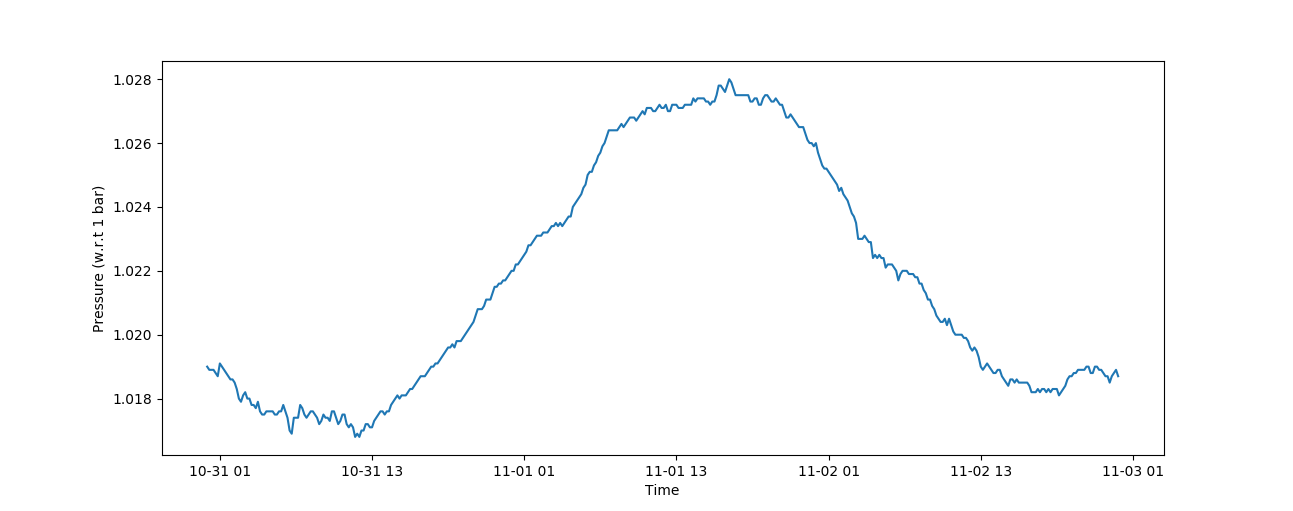
\includegraphics[width=\textwidth]{graphics/pressure_monitoring.png}
  \caption{Atmospheric pressure in Helsinki during the spectra measurement. Source: \cite{meteo}}
  \label{fig:pressure}
\end{figure}

Given the parameters and uncertainties quoted in table \ref{Tab:params}, a MC simulation was created in order to compute the theoretical uncertainties on the expected multiplication factor as a function of operating voltage. In this systematics treatment, each parameter was drawn out of gaussian shaped probability distribution, with a mean centered at a parameter's value and the width set as the quoted uncertainty. Figure \ref{fig:joker_plot} shows the 1$\sigma$ and 2$\sigma$ confidence interval of the multiplication factor, after propagation of systematic uncertainties.

The theoretical expectation for the drift chamber's electron yield can be compared to the data obtained during the iron spectrum scan described in section \ref{sec:voltage_calibration}. Given a number of MCA channels and an output voltage, the charge accumulated at the electrodes of the drift chamber can be obtained with equation \ref{eq:M_exp}.

\begin{equation}
  \label{eq:M_exp}
  Q_{detector} = \frac{V_{output}\cdot c_{preamplifier}}{G}
\end{equation}

where $G$ is the preamplifier gain and its associated uncertainty calculated in section \ref{preampcalib}. From that point, the multiplication factor of the experimental data is given by the following:

\begin{equation}
  M_{experimental} = \frac{Q_{detector}}{n_{Fe^{5}/Am^{241}}\cdot e}
\end{equation}

Where $n_{Fe^{5}/Am^{241}}$ is the average number of electrons-ion pairs produced bu either iron-55 (227) or americium-241 (2290), as taken from \cite{can_paper}.




\begin{table}[]
	\begin{tabularx}{\linewidth}{X|X|p{2cm}}
		\textbf{Element} & \textbf{Measurements} {[}mm{]}                                                  & \textbf{Size} \\ \hline
		Copper tube, length                        & $149.06$, $149.10$, $149.06$, $149.09$                                 &      \\
		Copper tube, wall thickness                & $1.04$, $1.00$, $1.02$, $1.02$, $1.02$, $1.14$, $1.05$, $1.04$, $1.04$ &      \\
		Copper tube, inner radius                  & $19.97$, $19.98$, $19.99$, $19.88$, $19.70$, $19.80$, $19.96$, $20.00$ &      \\
		Copper tube, radiation hole                & $5.03$, $5.04$, $5.08$                                                 &      \\
		Teflon HV front end,  total length         & $36.82$, $36.76$                                                       &      \\
		Teflon HV front end, top part length       & $15.91$, $15.94$, $15.86$                                              &      \\
		Teflon HV front end, tube extremity radius & $19.84$, $19.85$, $19.86$                                              &      \\
		Teflon back end, total length              & $15.04$, $14.97$, $14.89$, $14.93$, $14.95$, $15.06$                   &      \\
		Teflon back end, top part length           & $5.05$, $4.98$, $4.95$                                                 &      \\
		Teflon back end, tube extremity radius     & $19.88$, $19.86$                                                       &      \\
		Brass tube diameter                        & $1.0$                                                                  &      \\
		Anode wire thickened                       & $0.025$                                                                &     
	\end{tabularx}
\caption{Measurements of the copper pipe experiment setup components.}
\label{Tab:coppercan_sizes}
\end{table}
